In Versuch 255 setzen wir uns mit der Funktionsweise einer Röntgenröhre, sowie dem charakteristischen Spektrum der Röntenstrahlung auseinander. Neben quantitativen Untersuchungen des Röntgenspektrums selbst, nutzen wir das Prinzip der Bragg-Reflexion, um unter anderem die Gitterkonstante eines NaCl-Kristalls zu bestimmen.

\subsection{Physikalische Grundlagen}

\subsubsection*{Die Röntgenröhre}
Eine Röntgenröhre ist aufgebaut aus einer Glühkathode und einer Anode, welche sich in einem evakuierten Glaskolben befinden. Durch Glühemmission werden aus der Kathode Elektronen freigesetzt, welche durch eine Beschleunigungsspannung von $10$ bis $100\si{\kilo\volt}$, welche zwischen Kathode und Anode anliegt beschleunigt werden. Der kontinuierliche Teil des Röntgenspektrums wird durch die ausgehende Bremsstrahlung beim Abbremsen der Elektronen im Anodenmaterial verursacht. Diese Strahlung setzt bei einer bestimmten Grenzwellenlänge $\lambda_{gr}$ ein, welche sich nach
\begin{align}
  \lambda_{gr} = \frac{hc}{eU}\label{eq:grenzfreq}
\end{align}
berechnen lässt. Hierbei sind $h,c,e$ das Plank'sche Wirkungsquantum, die Lichtgeschwindigkeit und die Elementarladung. $U$ ist die an der Röntgenröhre anliegende Beschleunigungsspannung. Durch frei werdende Strahlung bei der Ionisation des Anodenmaterials ist dem kontinuierlichen Spektrum ein diskretes Spektrum überlagert, zu sehen in \abbref{fig:roentgenspektrum}, welches charakteristisch für das jeweilige Anodenmaterial ist. 

\begin{figure}[H]
  \centering
  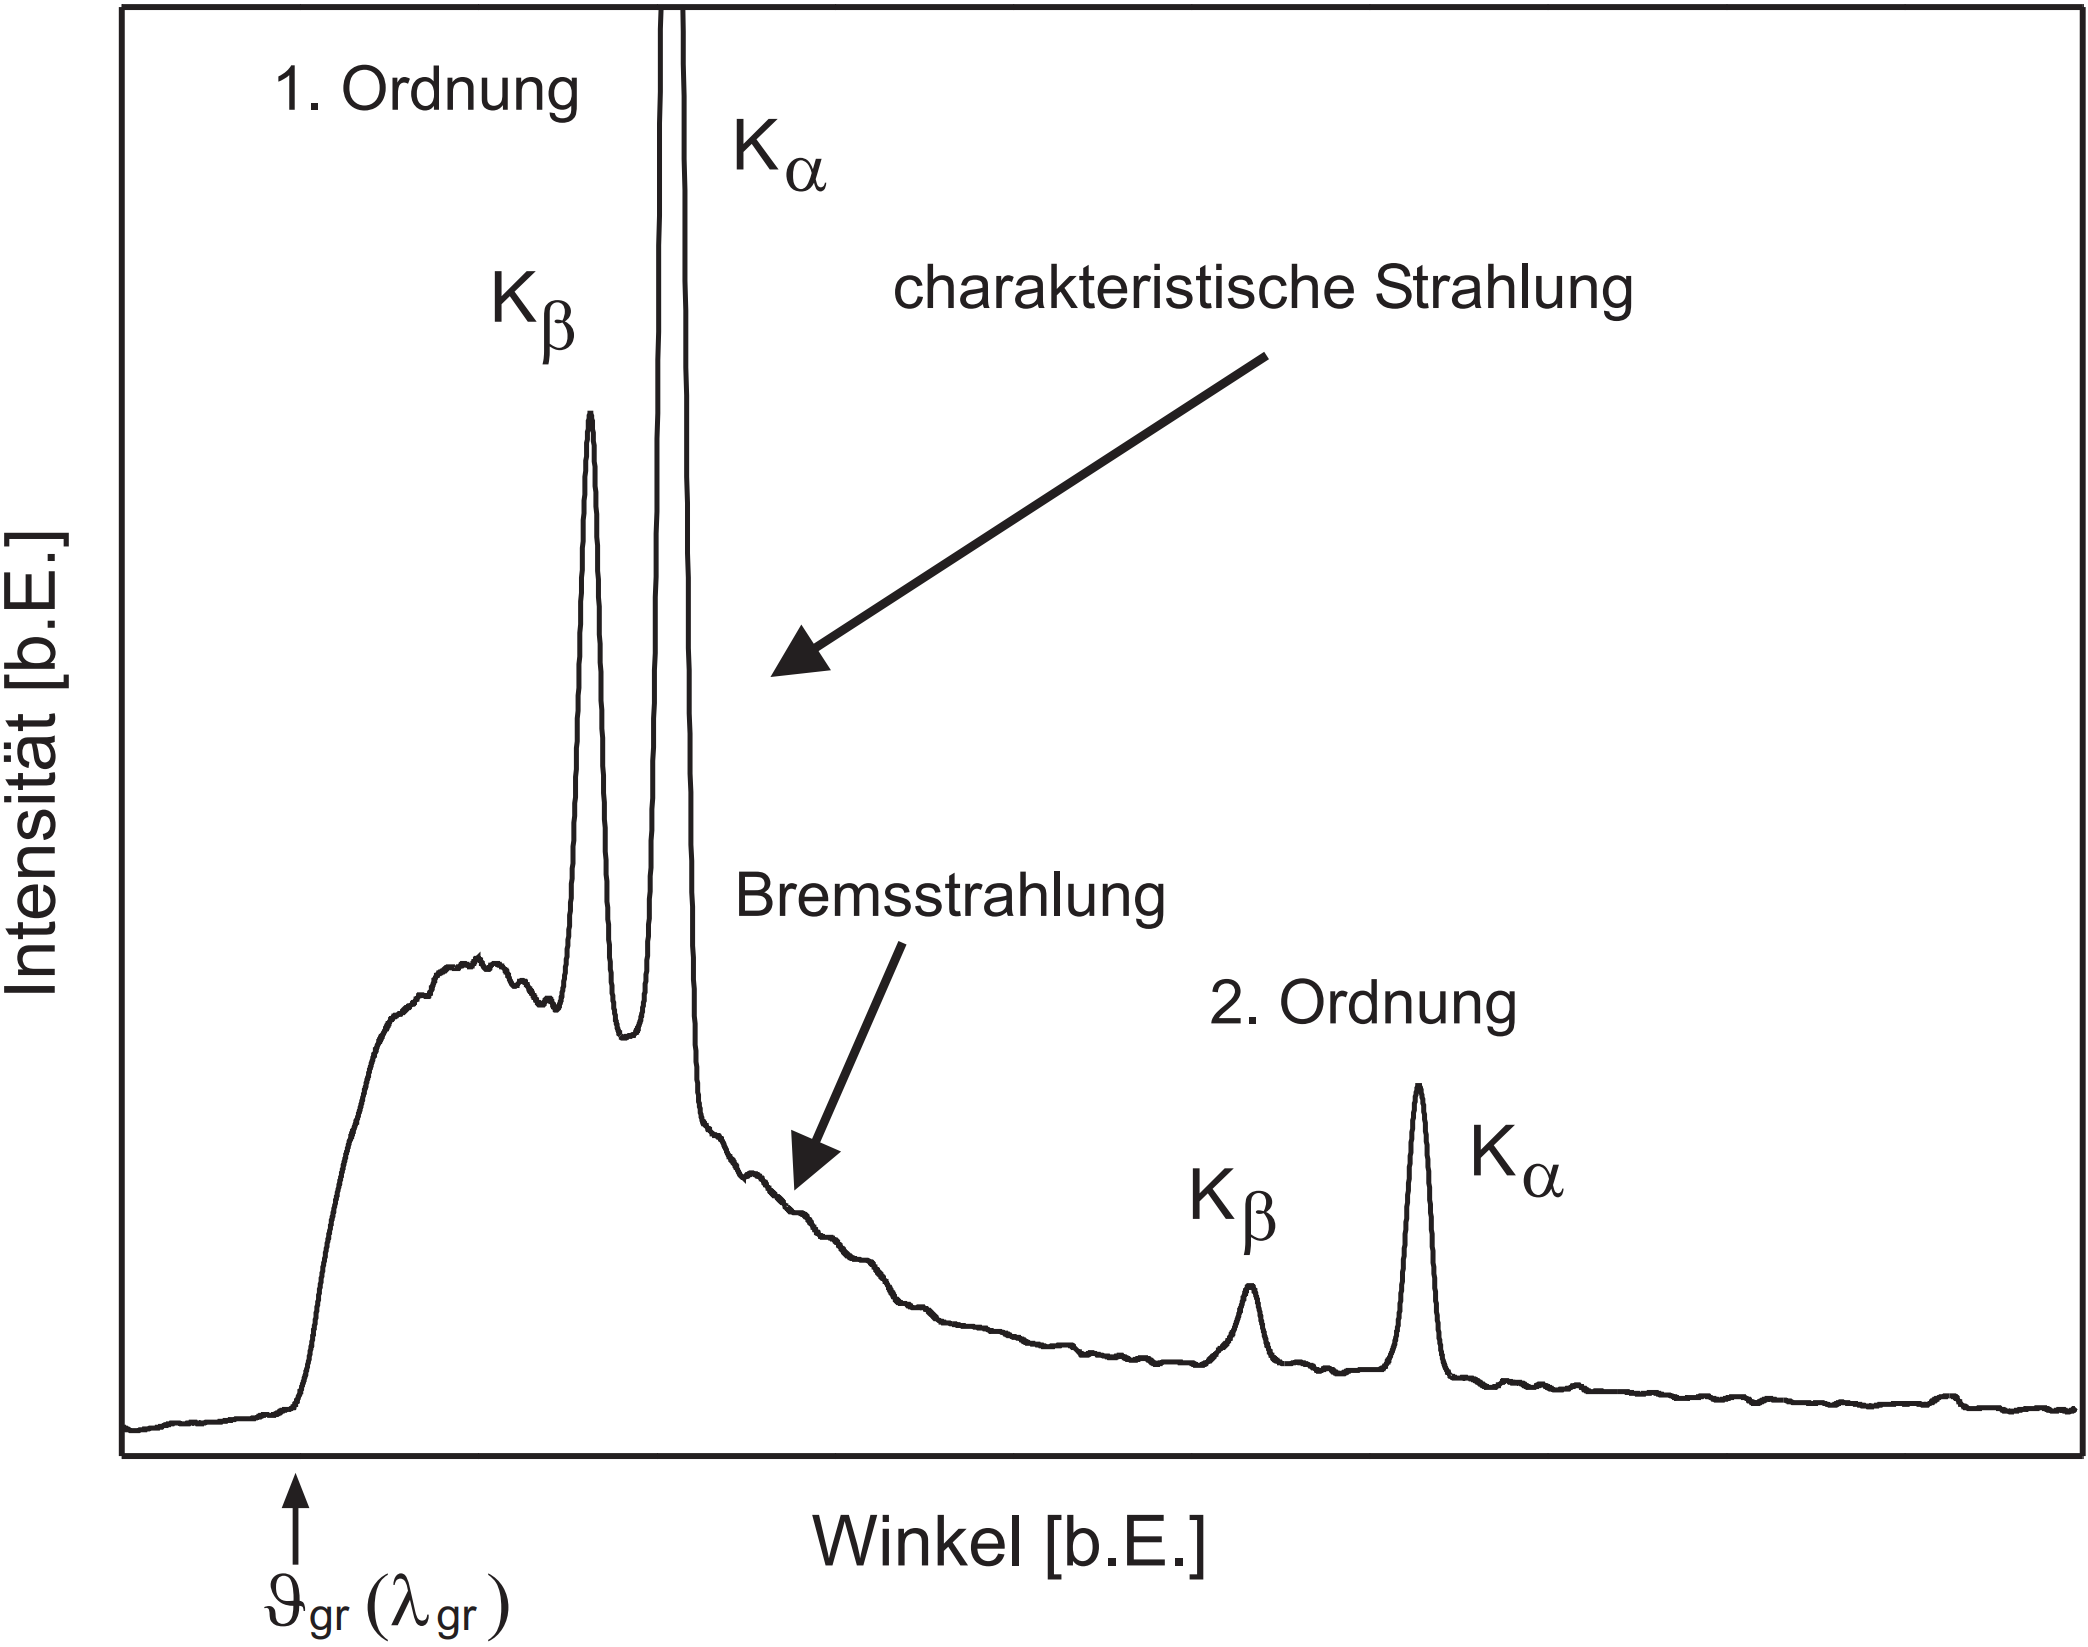
\includegraphics[width=.75\textwidth]{files/roentgenspektrum.png}
  \caption{Kontinuierliches und diskretes Röntgenspektrum.}
  \label{fig:roentgenspektrum}
\end{figure}

Die Positionen der Linien im diskreten Spektrum sind abhängig von der Ursprungs- und Ziel-Schale von bzw. zu welcher der Übergang des Elektrons stattfindet. Beispielsweise bezeichnen wir die Strahlung der Übergänge von der $L$- auf die $K$-Schale als $K_{\alpha}$-Strahlung, die für die Übergänge der $M$- auf die $K$-Schale als $K_{\beta}$-Strahlung. Die freiwerdende Energie eines Übergangs von der $n$-ten zur $m$-ten Schale lässt sich durch das Moseley'sche Gesetz
\begin{align}
  E_{n\to m} = hc R_{\infty} (Z-A)^2 \qty(\frac{1}{m^2} - \frac{1}{n^2})
\end{align}
berechnen. Hier gehen die Rydbergkonstante $R_{\infty}$, sowie die Kernladungszahl $Z$ und die Abschirmung der Kernladung als Abschirmungskonstante $A$ mit ein. Nähert man die Abschirmungskonstante als $A \approx 1$ an, so lässt sich mit dem Moseley'schen Gesetz eine näherung der Energie für die $K_{\alpha}$-Strahlung abhängig von der Kernladungszahl angeben:
\begin{align}
  E_{2 \to 1} = hc R_{\infty} (Z - 1)^2 \qty(\frac{1}{1}- \frac{1}{2^2}) = \frac{3}{4} hc R_{\infty} (Z - 1)^2.
\end{align}

Es ist zu beachten, dass bei genauerer Betrachtung, neben der Hauptquantenzahl, noch eine Entartung der Drehimpuls- und Spinquantenzahl in die freigesetzte Energie der Übergänge eingeht. Das Moseley'sche Gesetz gibt somit nur eine Näherung an.

\subsubsection*{Bragg-Reflexion}

Als Bragg-Reflexion bezeichnet man die Beugung von Röntenstrahlung durch die Gitterstruktur von Kristallen. Die Atomabstände in der Kristallstruktur befinden sich in der gleichen Größenordnung wie die Wellenlängen der Röntenstrahlung, weshalb sich die Bragg-Reflexion zur Untersuchung des Röntgenspektrums eignet. Die Bragg-Reflexion beruht darauf, dass auf den Kristall treffende Röntgenstrahlung sowohl an der Oberfläche, als auch den tieferliegenden Netzebenen der Kristallstruktur reflektiert wird. Beträgt der Gangunterschied $\Delta s = 2 d \sin(\vartheta)$ zweier Teilbündel, die unter dem Winkel $\vartheta$ eintreffen, siehe \abbref{fig:bragg_reflexion_drehkristall_a}, ein Vielfaches der Wellenlänge $\lambda$, so interferieren diese Konstruktiv, andernfalls destruktiv. Dies ist festgehalten durch das Bragg'sche Gesetz
\begin{align}
  2 d \sin(\vartheta) = n \lambda, \quad n \in \N. \label{eq:bragg}
\end{align}

\begin{figure}[H]
  \centering
  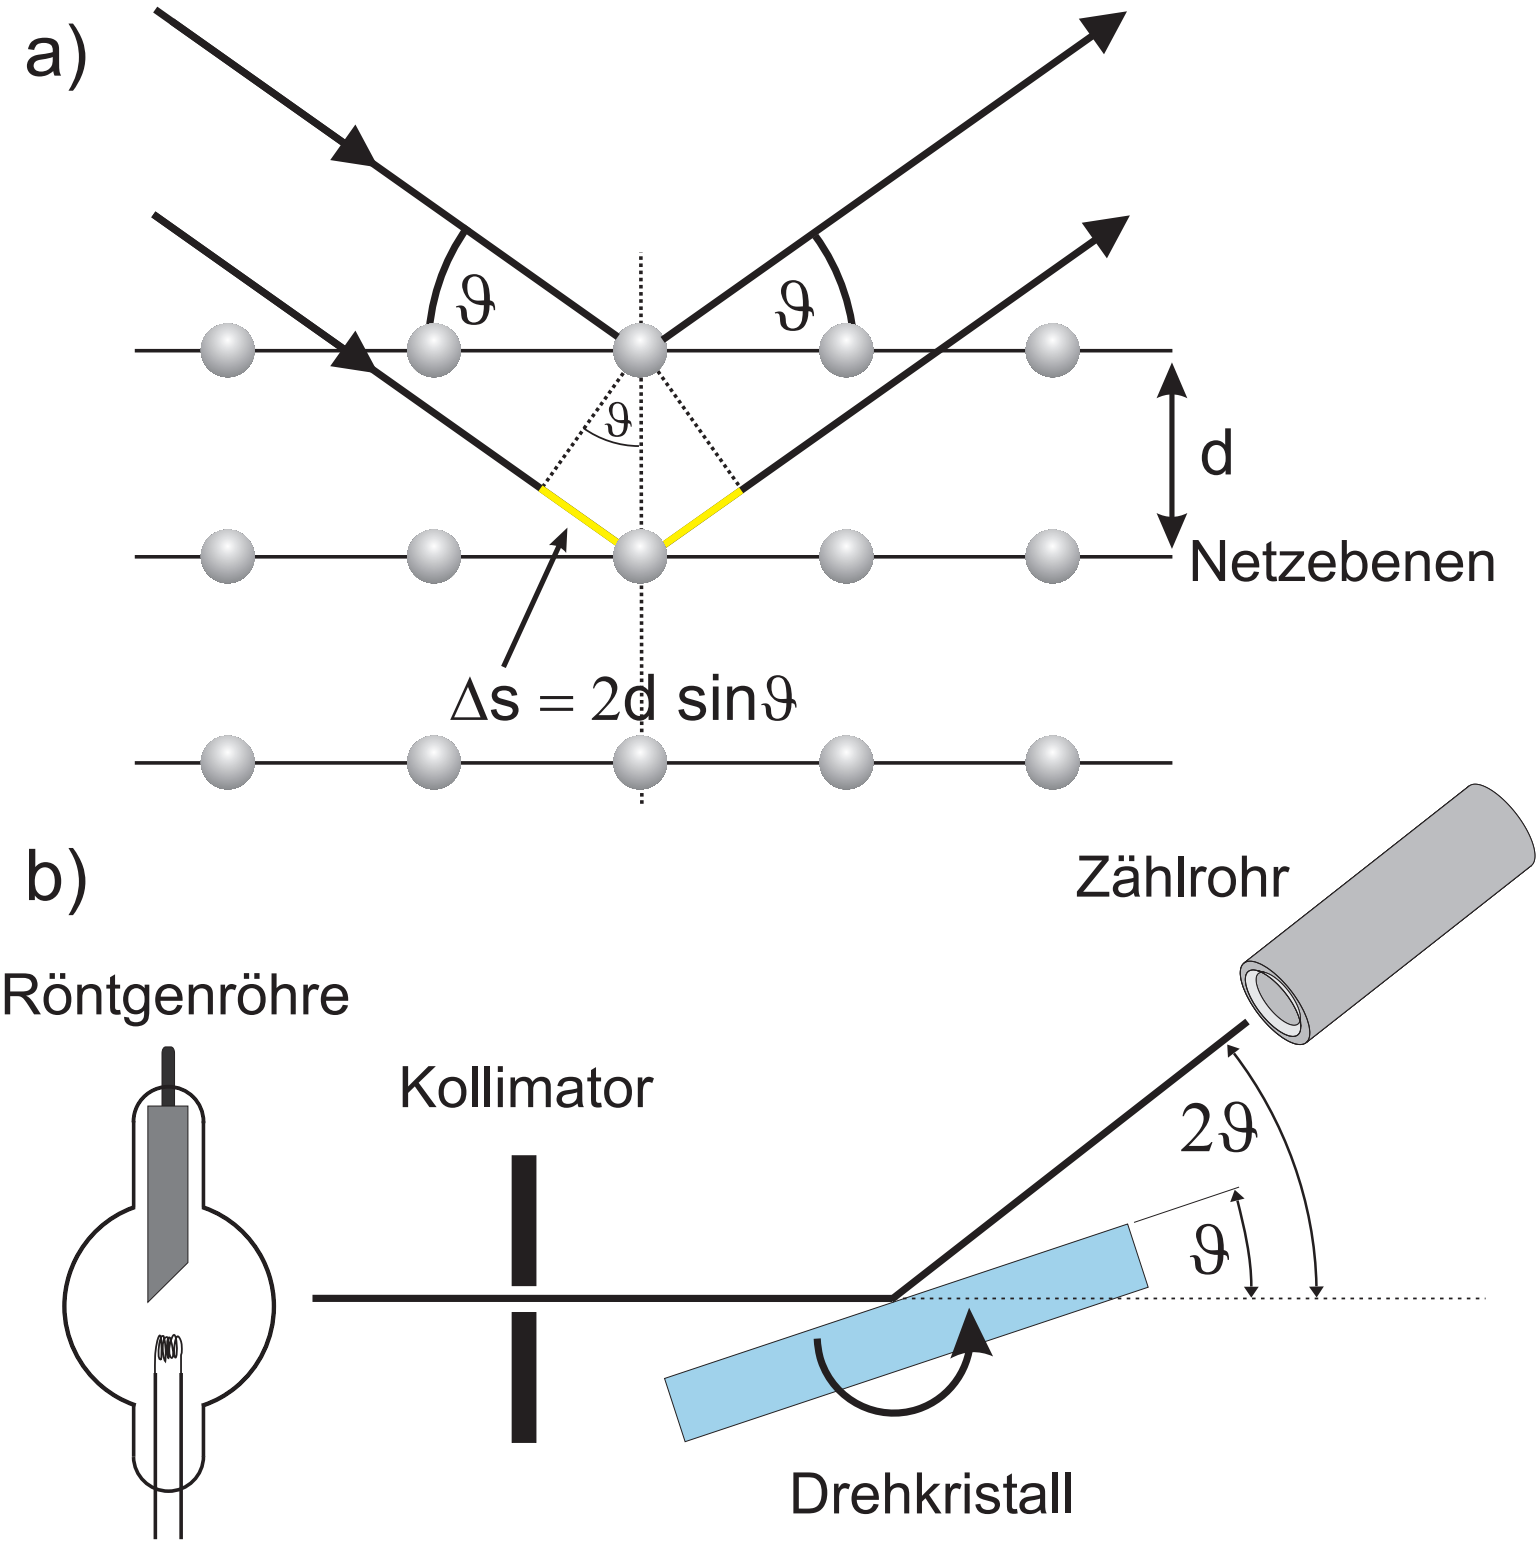
\includegraphics[width=.9\textwidth,trim={2cm 14cm 0.5cm 0},clip]{files/bragg_reflexion_drehkristall.png}
  \caption{Bragg-Reflexion von Röntenstrahlung an einem Kristall.}
  \label{fig:bragg_reflexion_drehkristall_a}
\end{figure}

Bei der sogenannten Drehkristallmethode wird diese Gesetzmäßigkeit angewandt. Dabei trifft Röntenstrahlung auf einen Kristall, welcher um die Achse senkrecht zu dieser gedreht wird. Welche Wellenlänge reflektiert wird, hängt dann gerade von der Winkelstellung des Kristalls ab. Die Intensität der reflektierten Strahlung kann dann mit einem Zählrohr gemessen und so Spektren wie in \abbref{fig:roentgenspektrum} aufgezeichnet werden. Ist der Drehkristall so justiert, dass gerade die Wellenlänge einer bekannten diskreten Linie reflektiert wird, lässt sich mit dem Bragg'schen Gesetz der Netzebenenabstand $d$ berechnen.

\subsubsection*{Kristallstruktur}

Kristalle sind aus sich periodisch wiederholenden Elementarzellen aufgebaut, wie sie Beispielsweise in \abbref{fig:elementarzelle_nacl_reordered} zu sehen sind. Bei NaCl- und LiF-Kristallen sind die drei Gitterkonstanten, also die Seitenlängen $a$ einer Elementarzelle, gleich groß.

\begin{figure}[H]
  \centering
  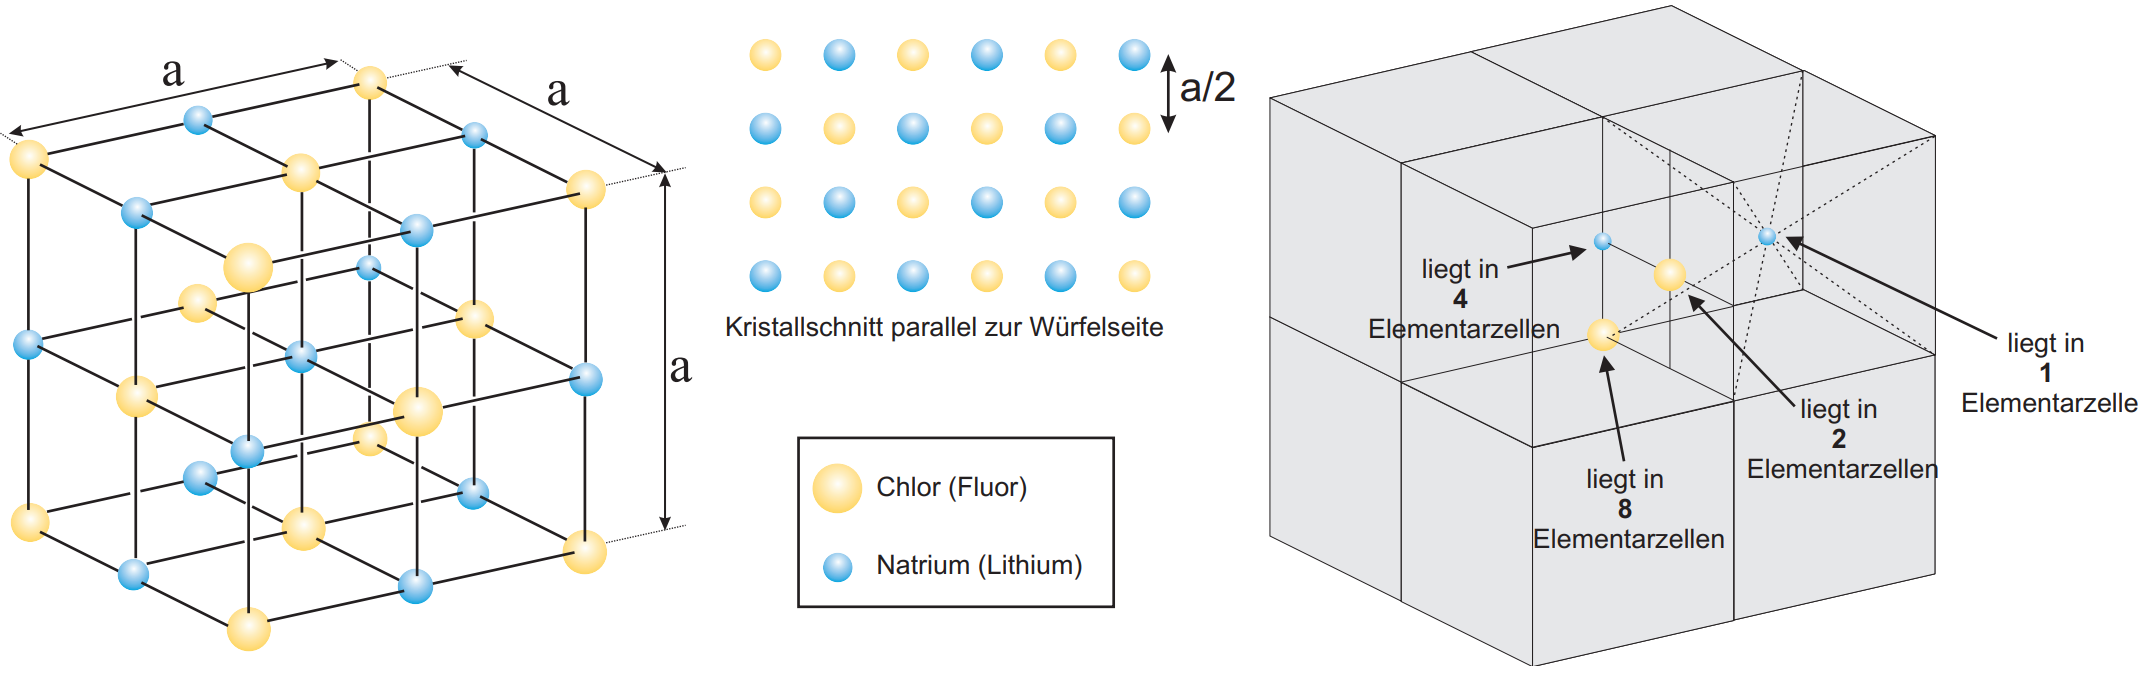
\includegraphics[width=\textwidth]{files/elementarzelle_nacl_reordered.png}
  \caption{Elementarzelle eines NaCl-Kristalls, deren periodische Anordnung, sowie der Kristallschnitt.}
  \label{fig:elementarzelle_nacl_reordered}
\end{figure}

Zur Ermittlung der Anzahl an Atomen, die einer Elementarzelle angehören, muss man beachten, zu wie vielen benachbarten Elementarzellen die Atome jeweils außerdem zählen. Dies ist ebenfalls in \abbref{fig:elementarzelle_nacl_reordered} dargestellt. Trägt ein Atom zu $x$ Elementarzellen bei, so zählt es für eine einzelne Elementarzelle nur zu $\flatfrac{1}{x}$. So lässt sich die Anzahl an Atomen am Beispiel der NaCl- (LiF-) Kristalle bestimmen.

\begin{table}[H]
  \centering
  \begin{tabular}{c|c|c|c||c|c}
    Element & Position & Beitrag zu x EZ & Beitrag zu einer EZ & Anzahl & Beitrag\\\hline
    Cl (F) & Ecken & $8$ & $\flatfrac{1}{8}$ & 8 & 1\\
    Cl (F) & Mitte Fläche & $2$ & $\flatfrac{1}{2}$ & 6 & 3\\
    Na (Li) & Mitte Kante & $4$ & $\flatfrac{1}{4}$ & 12 & 3\\
    Na (Li) & Mitte Zelle & $1$ & $\flatfrac{1}{1}$ & 1 & 1\\
  \end{tabular}
\end{table}

Aus den Beiträgen können ablesen, dass zu jeder Elementarzelle $4$ Chlor- (Fluor-) Atome und $4$ Natrium- (Lithium-) Atome, also $4$ NaCl- (LiF-) Moleküle, beitragen. Die Zahl $4$ geht bei der Berechnung der Avogadrokonstante wie folgt mit ein:
\begin{align}
  N_{A} = 4 \frac{V_{Mol}}{V}.
\end{align}
Dabei ist $V_{Mol}$ das Molvolumen eines einzelnen Moleküls und $V$ das Volumen einer Elementarzelle. Dieses lässt sich aus dem Netzebenenabstand $d$, welcher hier $\flatfrac{a}{2}$ beträgt, berechnen. Somit gilt
\begin{align}
  N_A = 4 \frac{V_{Mol}}{(2d)^3} = 4 \frac{M_{Mol}}{\rho (2d)^3} = \frac{1}{2}\frac{M_{Mol}}{\rho d^3}.\label{eq:avogadro}
\end{align}

\subsection{Versuchsdurchführung}

Zur Durchführung der Messungen verwenden wir ein Röntgengerät, welches mit einem Zählrohr-Goniometer ausgestattet ist (\abbref{fig:goniometer}). Die Röntgenstrahlung wird durch eine Röntgenröhre mit Molybdänanode erzeugt und über einen Kollimator auf den Drehkristall fokussiert. Das Zählrohr am Goniometer dreht sich im Verhältnis 2:1 mit dem Drehkristall, sodass es immer genau die Strahlung, welche im Winkel $\vartheta$ reflektiert wird erfassen kann.

\begin{figure}[H]
  \centering
  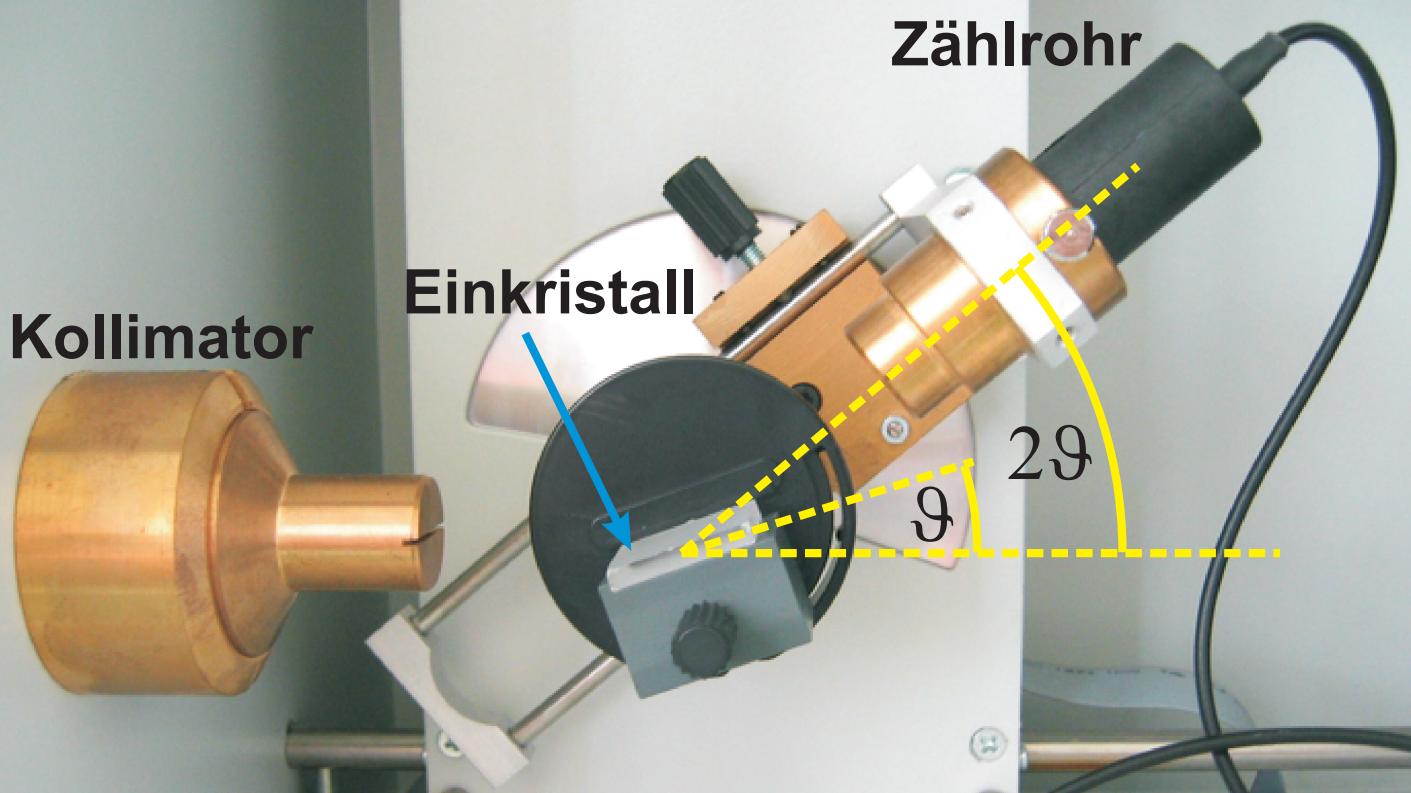
\includegraphics[width=.8\textwidth]{files/goniometer.png}
  \caption{Montierung des Drehkristalls und des Zählrohr-Goniometers im Winkelverhältnis 2:1.}
  \label{fig:goniometer}
\end{figure}

\textbf{Messung des Röntgenspektrums mit einem LiF-Kristall.} Bei einer Beschleunigungsspannung von $U = 35 \si{\kilo\volt}$, einem Strom von $I = 1\si{\milli\ampere}$ und einer Torzeit von $t = 5\si{\second}$ zeichnen wir das Röntgenspektrum in einem Winkelbereich von $3\si{\degree}$ bis $22\si{\degree}$ in $0.2\si{\degree}$-Schritten auf.

\textbf{Vermessen der $K_{\alpha}$ und $K_{\beta}$-Linien des Anodenmaterials.} Aus unseren Messdaten der vorherigen Aufgabe entnehmen wir die ungefähren Positionen der $K_{\alpha}$- und $K_{\beta}$-Linien. Mit den gleichen Einstellungen für Beschleunigungsspannung und Strom nehmen wir in deren Umgebung das Spektrum noch einmal in Winkelschritten von $0.1\si{\degree}$ und einer Torzeit von $20 \si{\second}$ auf.

\textbf{Zählrate als Funktion der Beschleunigungsspannung.} Bei einem festen Winkel von $7.5\si{\degree}$ Zeichnen wir die Zählrate für Beschleunigungsspannungen im Bereich von $20$ bis $35\si{\kilo\volt}$ in $1\si{\kilo\volt}$-Schritten jeweils über $20\si{\second}$ auf.

\textbf{Messung des Röntgenspektrums mit einem NaCl-Kristall.} Hier führen wir die Messung aus Aufgabe 1 noch einmal mit einem NaCl-Kristall in einem Winkelbereich von $3\si{\degree}$ bis $18\si{\degree}$ durch.